\section{Durchführung}
\label{sec:Durchführung}

Der Aufbau des Versuchs ist in Abbildung \ref{fig:aufbau} dargestellt.

\begin{figure}
  \centering
  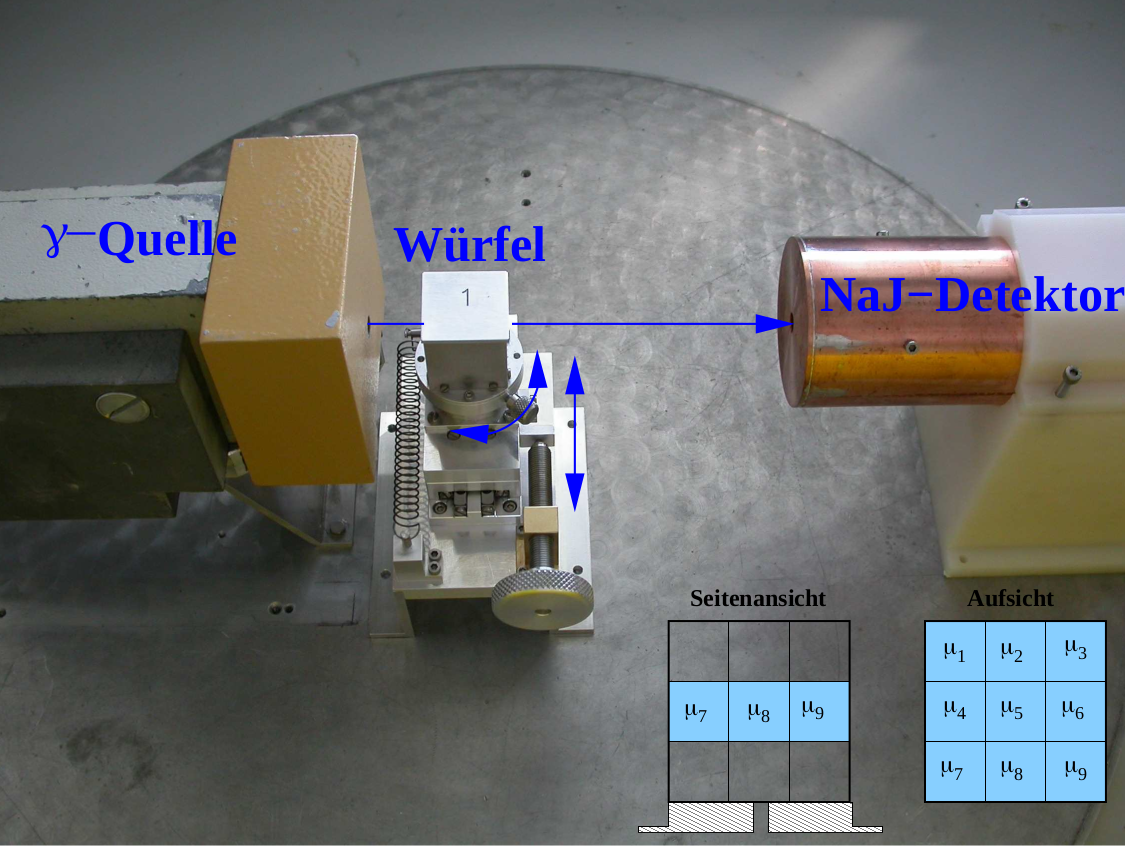
\includegraphics[width=\textwidth]{images/aufbau.png}
  \caption{Fotografie des Versuchsaufbaus. Links ist die Gammastrahlenquelle zu sehen. Der Strahlengang zum Detektor durch einen zu untersuchenden Würfel, der gedreht und in den Strahlengang hinein geschoben werden kann, ist eingezeichnet. \cite{Versuchsanleitung}.}
  \label{fig:aufbau}
\end{figure}

Dort ist links die Caesium-Probe, die die Gammastrahlung aussendet, zu sehen. Diese ist abgeschirmt, nur durch eine kleine Blende wird ein Strahl auf den zu untersuchenden Würfel kollimiert. Der Würfel befindet sich auf einer Apparatur, mit der er um seine $z$-Achse wie eingezeichnet gedreht werden kann, außerdem kann er in den Strahlengang herein und herausgedreht werden.

Das Energiespektrum wird mit einem Szintillationsdetektor aufgenommen, der hier durch einen $\ce{NaI}$-Detektor realisiert ist. Durch Streuung an den Atomen im Gitter dieses anorganischen Kristalls regt das einfallende und zu detektierende Gamma-Quant ein oder mehrere Elektronen, Löcher oder Elektronen-Loch-Paare (Exzitonen genannt) an, die sich durch den Kristall weiterbewegen. Dabei wird das Natriumiodid in der Regel mit Thallium dotiert, sodass die Bandstruktur geringfügig geändert wird. Rekombinieren die freigesetzten Teilchen bzw. Quasiteilchen an den sogenannten Aktivatorzentren, also den Fremdatomen, so rekombinieren diese dort und die Atome regen sich unter Aussendung von im Vergleich zu dem einfallenden Photon niederenergetischen Photonen über das sogenannte Aktivatorband ab. Die Photonenenergie ist dann zu niedrig, um ein Elektron vom Valenz- in das Leitungsband zu heben, sodass diese Photonen den Kristall zu einer ersten Photokathode passieren können, wo erste Elektronen ausgelöst werden.
Diese werden danach lawinenartig in einem Photomultiplier mithilfe eines Dynodensystems vervielfältigt. Bei den Dynoden handelt es sich um weitere Photokathoden, auf die die Elektronen mithilfe von elektrischen Feldern beschleunigt werden. Sie sind wegen ihrer Energiezunahme dann selbst in der Lage, weitere Elektronen auszulösen.

Die Impulshöhe des elektrischen Impulses aus den vervielfältigen Elektronen ist dann ein Maß für die Energie des am Anfang eingefallenen Gammaphotons. Um ein Energiespektrum zu erhalten, wird in diesem Versuch ein Multikanalanalysator verwendet. Dieser besteht aus einem Speicher mit einer bestimmten Anzahl an Kanälen. Die Impulshöhe des Signals wird bestimmt und der Speicher des Kanals um eins erhöht, dem die Impulshöhe am nächsten kommt. Dazu muss vorher ein Proportionalitätsfaktor definiert werden, mit dem die Energie in einen Kanal umgerechnet werden kann.
Im Versuch steht ein PC zur Verfügung, mit dem die Spektren digital ausgelesen werden können.

Es werden neben einer Nullmessung von $t=300$\,s vier verschiedene Würfel untersucht. Würfel 1 besteht lediglich aus einem Aluminiumgehäuse, das auch die äußere Schicht der weiteren Würfel bildet. Für diesen Würfel werden drei Projektionen für je $t=120$\,s gemessen. Würfel 2 und Würfel 3, die jeweils vollständig aus einem Material aus der Reihe Aluminium, Blei, Eisen, Messing und Delrin bestehen, werden für vier verschiedene Projektionen für jeweils $t=180$\,s vermessen. Würfel 4 wird für zwölf verschiedene Projektionen für je $t=180$\,s vermessen. Seine Elementarwürfel können aus den Materialien aus der obigen Reihe bestehen.
